
\PassOptionsToPackage{dvipsnames}{xcolor}
\documentclass[aspectratio=169,11pt]{beamer}

\newcommand{\teamname}{SWE Final Project Team}
\newcommand{\topicchoice}{Topic 1 -- Lost \& Found Matching Service}
\newcommand{\memberone}{Mahammad Javadzade}
\newcommand{\membertwo}{Teymur Alasgarov}
\newcommand{\memberthree}{Parvin Salahov}
\newcommand{\repolink}{https://github.com/ParvinSalahov/SWE-final-proj}
\newcommand{\coursecode}{AI-ENG-110}
\newcommand{\coursename}{Software Engineering}
\newcommand{\institution}{AI Academy, National AI Center}
\newcommand{\semester}{Spring 2026}

\usepackage[T1]{fontenc}
\usepackage[utf8]{inputenc}
\usepackage{xcolor}
\usepackage{tabularx}
\usepackage{booktabs}
\usepackage{listings}
\usepackage{tikz}
\usetikzlibrary{shapes.geometric,arrows.meta,positioning,fit,backgrounds}

\definecolor{accent}{HTML}{0B3D91}
\definecolor{soft}{HTML}{F2F4F8}
\definecolor{ok}{HTML}{166534}
\setbeamercolor{title}{fg=accent}
\setbeamercolor{frametitle}{fg=accent}
\setbeamercolor{section in head/foot}{bg=accent,fg=white}
\setbeamercolor{itemize item}{fg=accent}
\setbeamercolor{itemize subitem}{fg=accent}
\setbeamercolor{enumerate item}{fg=accent}
\setbeamercolor{block title}{bg=accent,fg=white}
\setbeamercolor{block body}{bg=soft,fg=black}
\setbeamerfont{title}{size=\Large,series=\bfseries}
\setbeamerfont{frametitle}{size=\large,series=\bfseries}
\setbeamerfont{footline}{size=\tiny}
\setbeamertemplate{navigation symbols}{}
\setbeamertemplate{footline}{%
  \leavevmode%
  \hbox{\hspace*{2ex}\tiny\textit{\teamname{} -- \topicchoice}\hfill%
  \tiny\textit{\coursecode{} -- \semester{}}\hfill%
  \tiny\insertframenumber/\inserttotalframenumber\hspace*{2ex}}%
  \vskip1pt%
}
\definecolor{codegreen}{rgb}{0,0.55,0}
\definecolor{codepurple}{rgb}{0.55,0,0.78}
\lstdefinestyle{python}{language=Python, backgroundcolor=\color{soft}, commentstyle=\color{codegreen}, keywordstyle=\color{accent}, stringstyle=\color{codepurple}, basicstyle=\ttfamily\scriptsize, breaklines=true, frame=single, framerule=0.4pt, rulecolor=\color{black!30}}

\begin{document}

{%
\setbeamertemplate{footline}{}
\begin{frame}[plain]
  \begin{center}
    \vspace{0.6cm}
    {\small \textsc{\institution}}\\[0.2em]
    {\small \textsc{\coursecode{} -- \coursename{} -- \semester{}}}\\[1.2em]
    \rule{0.7\textwidth}{0.6pt}\\[0.4em]
    {\Huge\bfseries\color{accent} \topicchoice}\\[0.4em]
    \rule{0.7\textwidth}{0.6pt}\\[1.2em]
    {\large \teamname}\\[0.6em]
    {\normalsize \memberone\quad\textbullet\quad\membertwo\quad\textbullet\quad\memberthree}\\[1cm]
    {\footnotesize\itshape Final Project Defense -- 2026-09-20}\\[0.4em]
    {\footnotesize\texttt{\repolink}}
  \end{center}
\end{frame}
}

\begin{frame}{The problem}
  \begin{block}{What the system does}
    Users report lost or found items with image and text, and the system ranks likely matches using VLM output plus embedding similarity.
  \end{block}
  \begin{columns}[T,onlytextwidth]
  \column{0.48\textwidth}
  \textbf{Inputs}
  \begin{itemize}
    \item item metadata: status, description, colors, attributes
    \item optional image file
  \end{itemize}
  \column{0.48\textwidth}
  \textbf{Outputs}
  \begin{itemize}
    \item structured item record
    \item embedding and match score
    \item ranked list of likely matches
  \end{itemize}
  \end{columns}
\end{frame}

\begin{frame}{Architecture}
  \begin{center}
  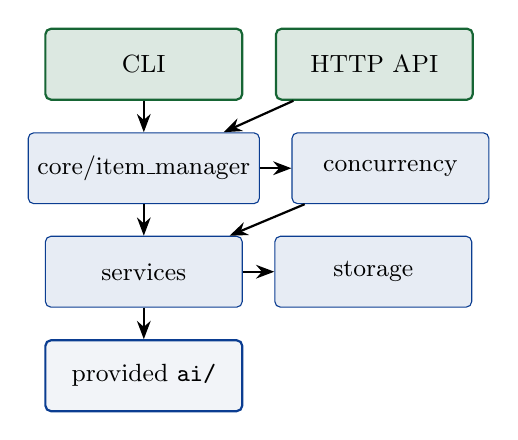
\begin{tikzpicture}[node distance=4mm, box/.style={draw,rounded corners=2pt,minimum width=2.5cm,minimum height=0.9cm,align=center,font=\small}, aibox/.style={box,fill=soft,draw=accent,thick}, sebox/.style={box,fill=accent!10,draw=accent}, entry/.style={box,fill=ok!15,draw=ok,thick}, arrow/.style={-Stealth,thick}]
    \node[entry] (cli) {CLI};
    \node[entry,right=of cli] (api) {HTTP API};
    \node[sebox,below=of cli] (core) {core/item\_manager};
    \node[sebox,right=of core] (conc) {concurrency};
    \node[sebox,below=of core] (svc)  {services};
    \node[sebox,right=of svc] (store) {storage};
    \node[aibox,below=of svc] (ai) {provided \texttt{ai/}};
    \draw[arrow] (cli) -- (core);
    \draw[arrow] (api) -- (core);
    \draw[arrow] (core) -- (conc);
    \draw[arrow] (core) -- (svc);
    \draw[arrow] (conc) -- (svc);
    \draw[arrow] (svc) -- (ai);
    \draw[arrow] (svc) -- (store);
  \end{tikzpicture}
  \end{center}
\end{frame}

\begin{frame}{Design decisions}
  \begin{enumerate}
    \item \textbf{Bounded async concurrency} -- we used \texttt{asyncio.Semaphore} to keep provider and DB calls under control.
    \item \textbf{Service boundary around AI} -- retries, validation, and caching are kept out of the UI layer.
    \item \textbf{Filesystem + database split} -- binary image data stays as files, metadata stays in the repository.
  \end{enumerate}
\end{frame}

\begin{frame}{Concurrency benchmark}
  \textbf{Workload:} batch of 10 mock item registrations.
  \begin{center}\small
  \begin{tabular}{lcc}
    \toprule
    & Sequential & Concurrent \\
    \midrule
    Wall-clock (s) & 0.5028 & 0.1009 \\
    Speedup & 1.0$\times$ & 4.98$\times$ \\
    \bottomrule
  \end{tabular}
  \end{center}
  \textbf{Why it matters:} the parallel design is a net win for bursty processing, while the semaphore keeps the work polite to external providers.
\end{frame}

\begin{frame}{Failure-mode story}
  \textbf{Scenario:} malformed or oversized image uploaded before AI description step.
  \begin{itemize}
    \item image is checked for length, magic headers, and Pillow decode validity
    \item invalid/unsafe input is rejected before the provider call
    \item no silent backend crash, no partial record persisted
  \end{itemize}
  \textbf{Result:} clearer logs, better user feedback, and a service that fails early and explicitly.
\end{frame}

\begin{frame}[fragile]{Docker demo}
  \textbf{Build the app:}
  \begin{lstlisting}[style=python,language=bash,numbers=none]
$ docker build -t lost-found-final .
$ docker run --rm --env-file .env lost-found-final python scripts/demo.py
  \end{lstlisting}
  \vspace{0.4em}
  \textbf{Start the database stack:}
  \begin{lstlisting}[style=python,language=bash,numbers=none]
$ docker compose up -d
$ docker compose exec app python scripts/demo.py
  \end{lstlisting}
\end{frame}

\begin{frame}{Testing and type checks}
  \begin{itemize}
    \item \texttt{pytest -q} → 82 passed in 1.44s
    \item \texttt{tests/test\_ai\_smoke.py} → 27 passed
    \item \texttt{mypy src tests scripts --python-version 3.12} → no errors
    \item \texttt{pyright src scripts tests} → 0 errors, 0 warnings
  \end{itemize}
\end{frame}

\begin{frame}{Limitations and next steps}
  \begin{itemize}
    \item benchmark isolates concurrency logic rather than full external-provider latency
    \item single-instance service, not a full distributed deployment
    \item rate-limit handling is local and retry-based, not queue-based
  \end{itemize}
  \textbf{If we had more time:} add richer observability, larger batch load tests, and a multi-provider failover strategy.
\end{frame}

\begin{frame}{Team contributions}
  \begin{center}\small
  \begin{tabularx}{\linewidth}{lXl}
    \toprule
    \textbf{Member} & \textbf{Primary work} & \textbf{Share} \\
    \midrule
    Mahammad Javadzade & storage, concurrency, benchmarking & 30\% \\
    Teymur Alasgarov & API + CLI + service flow & 38\% \\
    Parvin Salahov & tests, provider integration, validation & 32\% \\
    \bottomrule
  \end{tabularx}
  \end{center}
\end{frame}

{%
\setbeamertemplate{footline}{}
\begin{frame}[plain]
  \begin{center}
    \vspace{1cm}
    {\Huge\bfseries\color{accent} Questions?}\\[1.2em]
    \rule{0.5\textwidth}{0.6pt}\\[1.2em]
    {\large \teamname}\\[0.6em]
    {\normalsize \texttt{\repolink}}\\[1cm]
    {\footnotesize\itshape ``We can walk through any file in the repo.''}
  \end{center}
\end{frame}
}

\end{document}
